\chapter{Process}\label{chap:process}

The following chapter describes the processes used in the design and
implementation of the project. Section~\ref{sec:development-process}
provides and explanation of the development process and the approach
to implementation, and Section~\ref{sec:design-process} describes the
user-centred aspects of the design process.

\section{Development process}\label{sec:development-process}

A project with an individual developer requires a different approach
to time management than a multi-developer project. The lack of other
team members means that the development can afford to take a much more
flexible and dynamic approach, allowing for a faster pace and lower
cost of change in the development life cycle. Agile software processes
focus on this fast pace of change by encouraging frequent
communication with stakeholders and very short development iterations
\cite{highsmith2001agile, martin2003agile}.

Elements of the Agile manifesto \cite{fowler2001agile} inspired
decisions in the project development. For example, frequent meetings
with Dr Flower were used to provide ongoing feedback of development
progress, and meets the agile requirement for \textit{customer
  collaboration over contract negotiation}. Additionally, the
requirement for \textit{working software over comprehensive
  documentation} was used to justify the early development of a
working prototype which users could interact with, instead of lengthy
requirements notifications with potential users before beginning
development work. This resulted in useful design feedback during early
stages of the project development, as it is more intuitive for users
to provide feedback for a functional prototype then it is to discuss
requirements in a more abstract manner without being able to interact
with a product.

Not all of the Agile software philosophy was strictly adhered to. In
particular, the emphasis on \textit{responding to change over
  following a plan} was supplanted by the requirement for a formal
project plan document to be created in the first term. Since the Agile
philosophy doesn't provide a template or process for guiding
development, the iterative OpenUP development process was used to
provide a template for time management, by dividing the development
life cycle into discrete increments, each consisting of an inception,
elaboration, construction, and evaluation phase
\cite{balduino2007introduction}. OpenUP was chosen for the development
process due to its entirely open source nature as part of the Eclipse
Process Framework, and because it targets small teams and agile
development by design \cite{kroll2006agility}. Development was split
over three iterations, with one covering the first term, and two in
the second term. The end of each iteration's evaluation phase
culminated in a design and implementation milestone pair.

\subsection{Version Control}\label{subsec:version-control}

The git version control system was used to provide version control. A
single monolithic git repository tracks revisions for all pip-db
source codes and associated data. By using version control from the
very first day of the project, a fully accountable and transparent
history of the project's development has been recorded, with 2,392
revisions committed since 14 October 2013.

Git was chosen as the version control system due to it's support for
lightweight branching and it's distributed-by-design nature
\cite{chacon2009pro}. While the benefits of distributed version
control are not entirely exploited for single-developer projects, the
support for concurrent development of branches encourages
experimentation and an agile approach to development.

\subsection{Open Source}\label{subsec:open-source}

One of the key considerations of the project objectives
(Section~\ref{sec:objectives}) was that the finished project should be
freely available without commercial interest, and this extends to the
source code and development process. The success of truly open models
of development have investigated in great detail
\cite{weber2004success, godfrey2000evolution, chesbrough2006open,
  von2005democratizing}, and a philosophy of ``release early, release
often'' has been encouraged in open source communities as a technique
for nurturing rapid and widespread user involvement from an early
stage \cite{raymond1999cathedral}. As a result, all of the program
code, documentation and supporting files that have been created for
pip-db have been released under the terms of the GNU General Public
License v3 \cite{gnu2007gpl}. This is an open and permissive license
that allows for commercial use, but it mandates that derivative works
maintain the same license and must distribute the source code openly.

The combination of open source license and the use of git version
control meant that the online project hosting could be used to provide
a public centre for development. For this, the GitHub website was
used, which is the most popular online repository hosting site
\cite{finley2011github}, and offers free hosting for open source
projects.

%%%%%%%%%%%%%%%%%%%%%%%%%%%%
%% Figure: github-project %%
%%%%%%%%%%%%%%%%%%%%%%%%%%%%
\begin{figure}[H]
\centering
    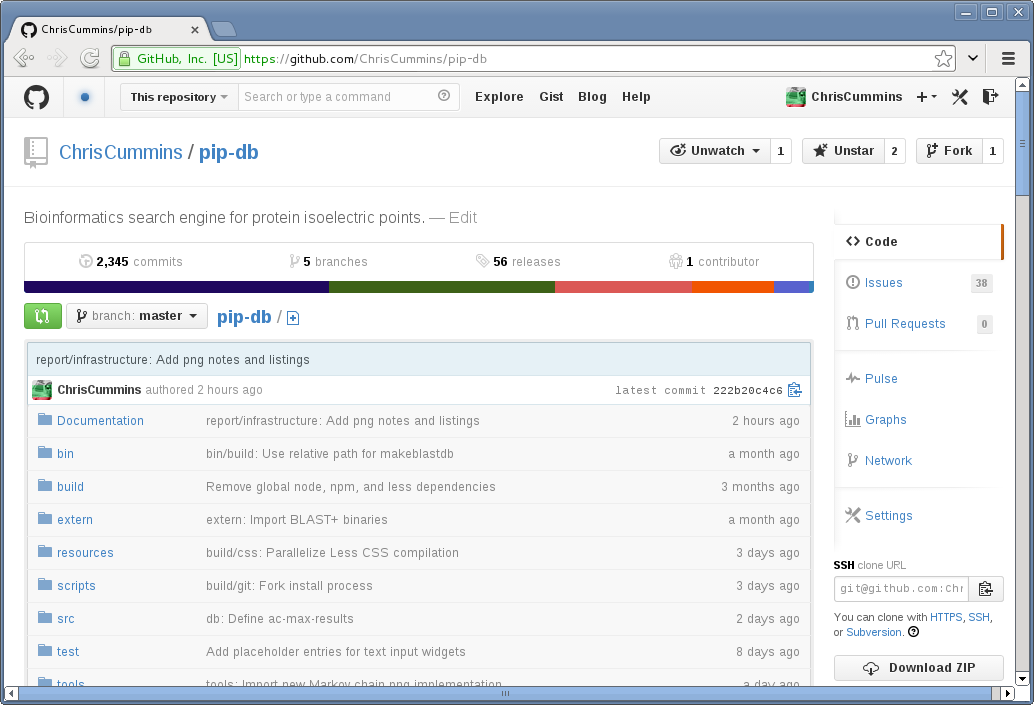
\includegraphics[width=0.82\textwidth]{assets/github}
\caption[GiHub project homepage]
        {Screenshot of the GitHub page for the pip-db repository.}
\label{fig:github-project}
\end{figure}

\subsubsection*{A note on dataset confidentiality}
It is important to note that while pip-db is an open source project,
the PIP-DB dataset as supplied by Dr Flower remains confidential,
and so has not been released for distribution at his request.

\subsection{Development workflow}\label{subsec:github-workflow}

In addition to hosting the project source code and revision history,
GitHub provides many useful features intended for collaborative
development efforts, including an issue tracker, milestones, and a
Wiki. By combining these features with strict version control
practises, it is possible to create a dynamic development environment
which simultaneously encourages experimentation and rapid change while
providing a full history of changes and the ability to roll back and
integrate new features when required.

The issue tracker provided by GitHub was used from the project
inception. The purpose of the issue tracker is to document requests
for changes. Whilst the revision control log provides a history of all
of the changes which have been made, the issue tracker is used as a
place to document changes which \textit{should} be made, but not have
not yet been completed. Each issue is assigned a unique identifier,
and these identifiers can be used in revision messages to provide a
cross reference between the revision control history and the known
issues and bugs. In total, 350 issues have been opened, of which 39
remain open at the time of writing.

Issues can be categorised using labels
(Table~\ref{tab:issue-labels}). Labels provide additional meta data
regarding a type of issue, and each issue can be assigned multiple
labels. The issue tracker can filter issues by labels, allowing for a
quick visual overview of the issues particular types.


%%%%%%%%%%%%%%%%%%%%%%%%%%%
%% Figure: github-issues %%
%%%%%%%%%%%%%%%%%%%%%%%%%%%
\begin{figure}[H]
\centering
    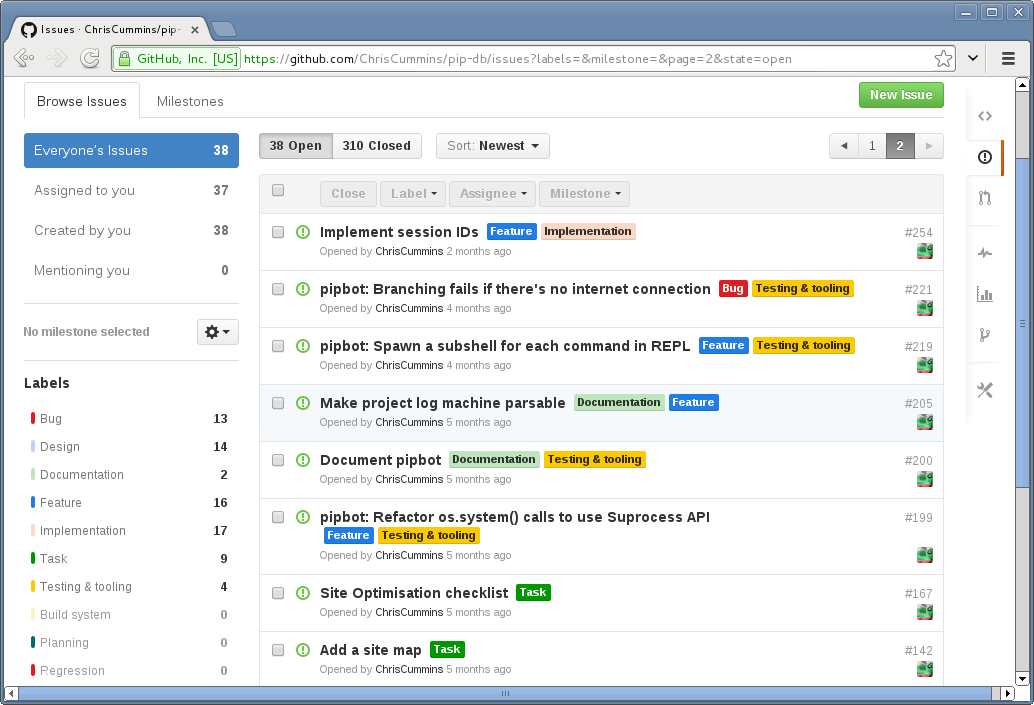
\includegraphics[width=0.82\textwidth]{assets/github-issues}
\caption[GitHub project open issues]
        {Screenshot of GitHub's issue tracker for pip-db.}
\label{fig:github-issues}
\end{figure}


%%%%%%%%%%%%%%%%%%%%%%%%%
%% Table: issue-labels %%
%%%%%%%%%%%%%%%%%%%%%%%%%
\begin{table}[H]
\centering
\begin{tabular}{l l}
\textbf{Label} & \textbf{Description}\\
\hline
Bug & Crash reports, stack traces, and software failures.\\
Design & Issues relating to the user interface design.\\
Documentation & Documentation tasks.\\
Feature & Web service feature addition requests.\\
Implementation & Issues relating to the web server implementation.\\
Task & Feature addition requests.\\
Testing \& tooling & Issues relating to infrastructure.\\
Build system & Bugs and issues with the build system.\\
Planning & Issues relating to TP1 project planning.\\
Regression & Issues which have arisen as a result of changes, not additions.\\
Version control & Git and GitHub issues and feature requests.\\
Wontfix & Used to indicate issues which have been closed without being fixed.\\
\end{tabular}
\caption[Issue tracker labels]
        {The labels used for categorising issues, and their corresponding meanings.}
\label{tab:issue-labels}
\end{table}


In addition to assigning labels to issues, GitHub also supports the
creation of milestones with set dates. Issues can be assigned to
milestones, and the number of open and closed issues per milestone can
be shown, providing an indication of the progress towards a particular
milestones (Figure~\ref{fig:github-milestones}.


%%%%%%%%%%%%%%%%%%%%%%%%%%%%%%%
%% Figure: github-milestones %%
%%%%%%%%%%%%%%%%%%%%%%%%%%%%%%%
\begin{figure}[H]
\centering
    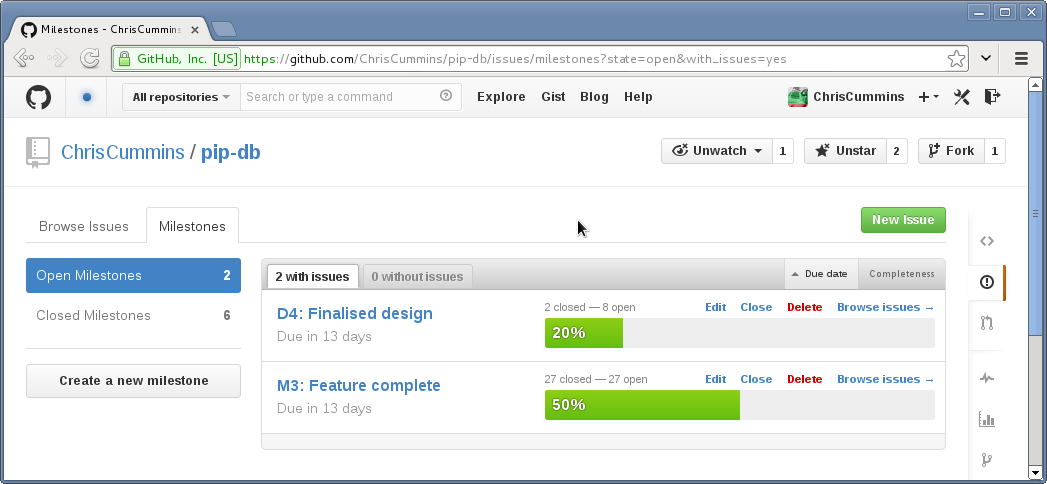
\includegraphics[width=0.82\textwidth]{assets/github-milestones}
\caption[GitHub project open milestones]
        {Screenshot of GitHub's milestones overview for pip-db.}
\label{fig:github-milestones}
\end{figure}


\subsection{Branching model}

A branching model was designed for this project in order to provide a
consistent branching and release strategy to use over the course of
development. Since the revision control must track a huge number of
changes (over 2000) over the course of several months, it is important
that the revision history be as clear as possible, and that branches
are used intelligently to provide additional information about the
project development, not to obscure past work.

The branch model that I was designed was inspired by Driessen's
\textit{Successful Git branching model} \cite{driessen2012successful},
with a number of changes to adapt it specifically for this
project. The core of Driessen's model is two permanent branches which
track the current development head, and the latest stable
release. Developers work on the development branch, and update the
stable branch at release time. Transient auxiliary branches are used
as staging areas for new features and releases. The hotfix branch
support was removed from Driesson's model, since the software
developed is only proof and concept and so does not need to support
regression patching.

Importantly, the name scheme for feature branches was changed so that
it matched the GitHub issue IDs. This meant that work on a feature
should only begin when it has an open issue assigned to it, enforcing
the use of the issue tracker. This novel integration of issue tracker
and version control system means that for every change made in the
project, it is possible to trace back not only the revision which
introduced the change, but also the issue or feature request which
demanded the change. This means that every change is justified with a
reason \textit{why} the change was made not, not just the description
of \textit{how} the change was made which is provided by the revision
history.


%%%%%%%%%%%%%%%%%%%%%%%%%
%% Table: branch-names %%
%%%%%%%%%%%%%%%%%%%%%%%%%
\begin{table}[H]
\centering
\begin{tabular}{l l L{8cm}}
\textbf{Driesson} & \textbf{Cummins} & \textbf{Purpose}\\
\hline
\texttt{master} & \texttt{stable} & The latest stable release.\\
\texttt{develop} & \texttt{master} & The current development head.\\
\texttt{release/:name} & \texttt{release/:version} & Release candidate staging areas.\\
\texttt{feature/:name} & \texttt{wip/:id} & Feature addition branches (cross referenced with issue tracker using issue IDs).\\
\texttt{hotfix/:name} & & Hotfix development branches.\\
\end{tabular}
\caption[Development model branch names]
        {A comparison of branch names with Driesson's development model.}
\label{tab:branch-names}
\end{table}


\section{Design process}\label{sec:design-process}


\subsection{User-centred design}\label{subsec:user-centred-design}

% Existing systems

\cite{lu2011pubmed, hearst2007biotext}

% CRITIQUE of Darren's systems

% Usability research

\cite{bolchini2009better, pavelin2012bioinformatics}


\subsection{Low fidelity prototyping}\label{subsec:low-fidelity-prototype}

% TODO: Low-fi
\cite{egger2000lofi}

% TODO: Balsamiq


\subsection{High fidelity prototyping}\label{subsec:high-fidelity-prototype}

% TODO: Rapid prototyping using PHP + CSS + HTML + JS

% TODO: Both DESIGN and TECHNICAL prototype
